We consider the behavior of the logistic equation under the presence of noise, in multiplicative way to the population. For the elements $(t,x)\in Q=(0, T)\times(0, M)$, we state the following differential equation,
\begin{equation}
	dx=\left(rx\left(1-\frac{x}{M}\right)\right)\diff{t}+\sigma x\diff{W} \label{eq: Constant Harvesting Stochastic}
\end{equation}

A unique solution exists if both It\'o conditions hold (Fleming and Rishel, 1975). The first one is the linear growth condition, for some independent constant $K$,
\begin{align}
	\abs{rx\left(1-\frac{x}{M}\right)}&\leq K\left(1+\abs{x}\right) \label{eq: LinearGrowth Det}\\
	\abs{\sigma x}&\leq K\left(1+\abs{x}\right) \label{eq: LinearGrowth Stoch}
\end{align}
The second one is the Lipschitz condition,$\exists L$ independent constant, and $\forall x$, $\exists B(x)$ neighborhood of $x$, such that $\forall x_1, x_2 \in B(x)$,
\begin{align}
\abs{rx_2\left(1-\frac{x_2}{M}\right)-rx_1\left(1-\frac{x_1}{M}\right)}&\leq L \abs{x_2-x_1} \label{eq: Lipschitz Det}\\
\abs{\sigma\left(x_2-x_1\right)} &\leq L \abs{x_2-x_1} \label{eq: Lipschitz Stoch}
\end{align}

Since $F(x,t)=rx\left(1-\frac{x}{M}\right)$ is continuously differentiable in $x$, $F$ is Lipschitz in $x$ then condition \ref{eq: Lipschitz Det} is satisfied. For bounded $\sigma$, condition \ref{eq: Lipschitz Stoch} is satisfied. Moreover the sufficient conditions for the It\^o conditions are satisfied for all functions $C^1$ on the closure of any compact set $Q$.

Since the above conditions are satisfied, we can guarantee existence and uniqueness of the solution for the equation \ref{eq: Constant Harvesting Stochastic}. Given by the equation:
\begin{equation}
\begin{array}{lll}
	x(t)&=&x_0+\int_{0}^{t}\left(rx\left(1-\frac{x}{M}\right)-u\right)\diff{t} + \int_{0}^{t}\sigma x \diff{W},\\
	x(0)&=&x_0, \\
	W(0)&=&0.
\end{array}
\end{equation}


\begin{figure}[H]
	\centering{
	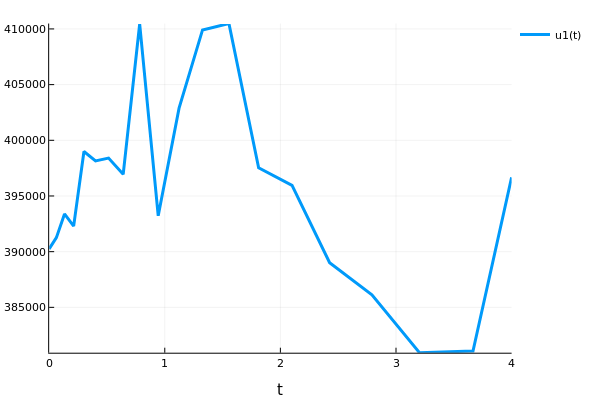
\includegraphics[width=0.6\textwidth]{Noise1.png}
	}
	\caption{Simulation performed of logistic equation \ref{eq: Constant Harvesting Stochastic}, with parameters $r=0.8\frac{1}{\text{month}\times\text{fish}}$, $x_0=\frac{M}{2}$, for a population in natural conditions (harvest exploitation $u=0$.), with presence of noise proportional to the population, with $\sigma=0.1$. Performed during 4 months.  }
\end{figure}


